\documentclass{ltjsarticle}

\usepackage{mathtools}
\usepackage{siunitx}
\usepackage{listings}
\usepackage{graphicx}
\usepackage{xcolor}
\usepackage{multirow}
\usepackage{url}
\usepackage[%
	backend=bibtex,
	citestyle=numeric,
	url=true,
	doi=true,
	bibencoding=utf8,
	bibstyle=ieee,
	]{biblatex}
\addbibresource{Python1.bib}
\definecolor{listinggray}{gray}{0.9}
\setlength{\columnseprule}{0.4pt}
\lstset{%
	stringstyle=\ttfamily,
	columns=fullflexible,
	numbers=left,
	numberstyle={\tiny \emph},
	numbersep=5pt,
	frame=single,
	morecomment=[l]{//},
}
\renewcommand{\lstlistingname}{ソースコード}

\begin{document}

\section{目的}
Pythonのライブラリについて理解を深め、画像処理技術の第一歩を学ぶとともに、基本となるOpenCVの基礎的な使い方を学ぶ。

\section{理論}

\subsection{平滑化フィルタ}
平滑化フィルタはノイズの低減やぼかしなどを行う、基本的なフィルタ処理の一つである。

あるピクセルを中心として\(3\times3\)などの大きさのオペレーターを置く。
そしてオペレーター内のピクセル値の平均をそのピクセルの値とすることで、画像全体がぼやけたような効果が得られる。

ランダムノイズの低減に効果的だが、画像のディテールやエッジも同時にぼやけてしまう性質がある。

\subsection{中央値フィルタ}
中央値フィルタもノイズ除去を行うフィルタ処理の一種だが、平滑化フィルタとは違い塩胡椒ノイズに強いという性質がある。

平均化フィルタと同じようにオペレーターを置き、オペレーター内のピクセル値の中央値を中心のピクセルの値とする。

この手法はエッジや細部の値をあまり変えることなくノイズを除去でき、計算も比較的容易である。
しかしオペレーターが大きすぎると細部が失われてしまうことや塩胡椒ノイズ以外に効果が薄いことが欠点である。

\subsection{特徴検出の仕組み}

\subsubsection{グレースケール化}
画像全体をグレースケール化して画像処理をより行いやすくする。

\subsubsection{ノイズ除去}
平滑化フィルタや中央値フィルタを使いノイズを除去して、より特徴検出をしやすくする。

\subsubsection{二値化とネガポジ反転}
しきい値を決めそれを使って画素を白と黒に分ける処理を画像全体に行う。
この時ヒストグラムを使うことでしきい値の調整がやりやすくなる。

その後特徴検出のため白と黒の画素値を反転するネガポジ反転を行う。

\subsubsection{特徴検出}
しきい値の調整がうまくいくと連続した塊が表れる。
これをブロブという。
ブロブを囲む円や長方形、ブロブの面積や輪郭、形状などを調べることで物体の特徴を検出できる。

\subsection{エッジ検出}
ラプラシアンフィルタやガウシアンフィルタのようにオペレーターの値を調整することで物体のエッジを検出することができる。

\subsection{ハフ変換}
ハフ変換という特徴検出手法がある。 %直線のハフ変換
ある直線上にある点の座標を\((x,y)\)としてそれをパラメータ空間\((\rho,\theta)\)に映す。
その点を通る直線に対し\(\rho\)を原点からの距離、\(\theta\)をX軸と距離がなす角度としたとき式\ref{eq:HesseNormalForm}と表せる。
これをヘッセの標準形という。
\begin{align}
	\rho = x\cos\theta + y\sin\theta \label{eq:HesseNormalForm}
\end{align}
この式を満たす\((\rho,\theta)\)は無数に存在するのでパラメータ空間では正弦波が表れる。
この処理をエッジの点全体にかけることで重なる点が出てくる。
その中で投票をし一番得票数の多かった点\((\rho,\theta)\)をある直線の距離と角度として検出する。

円のときも円上の点\((x,y)\)に対して同じ処理をすることで円を検出できる。 %円のハフ変換
このとき円の中心座標\((p,q)\)と半径\(r\)で式\ref{eq:HoughCircle}と表せる。
\begin{align}
	r ^ 2 = (x - p) ^ 2 + (x - q) ^ 2 \label{eq:HoughCircle}
\end{align}

\section{方法}

\subsection{物体検出}
画像に平均化フィルタと中央値フィルタの両方をかけたあと、画素値のヒストグラムを作りそれを参考に二値化を施しネガポジ反転する。
そしてBoundingRect関数とrectangle関数を使って長方形を描く。

\subsection{円検出}
OpenCVライブラリの機能であるCanny関数とHoughCircles関数を使ってハフ変換を行う。
そこから中心点の座標と半径を得てCircle関数を使い円を描く。

\section{結果}

\subsection{物体検出}
結果は図\ref{fig:img_org}~\ref{fig:img_res}のようになった。
ソースコードはコード\ref{src:SquareCode}

\begin{figure}[htbp] %物体検出の結果画像
	\begin{minipage}{0.23\linewidth}
		\centering
		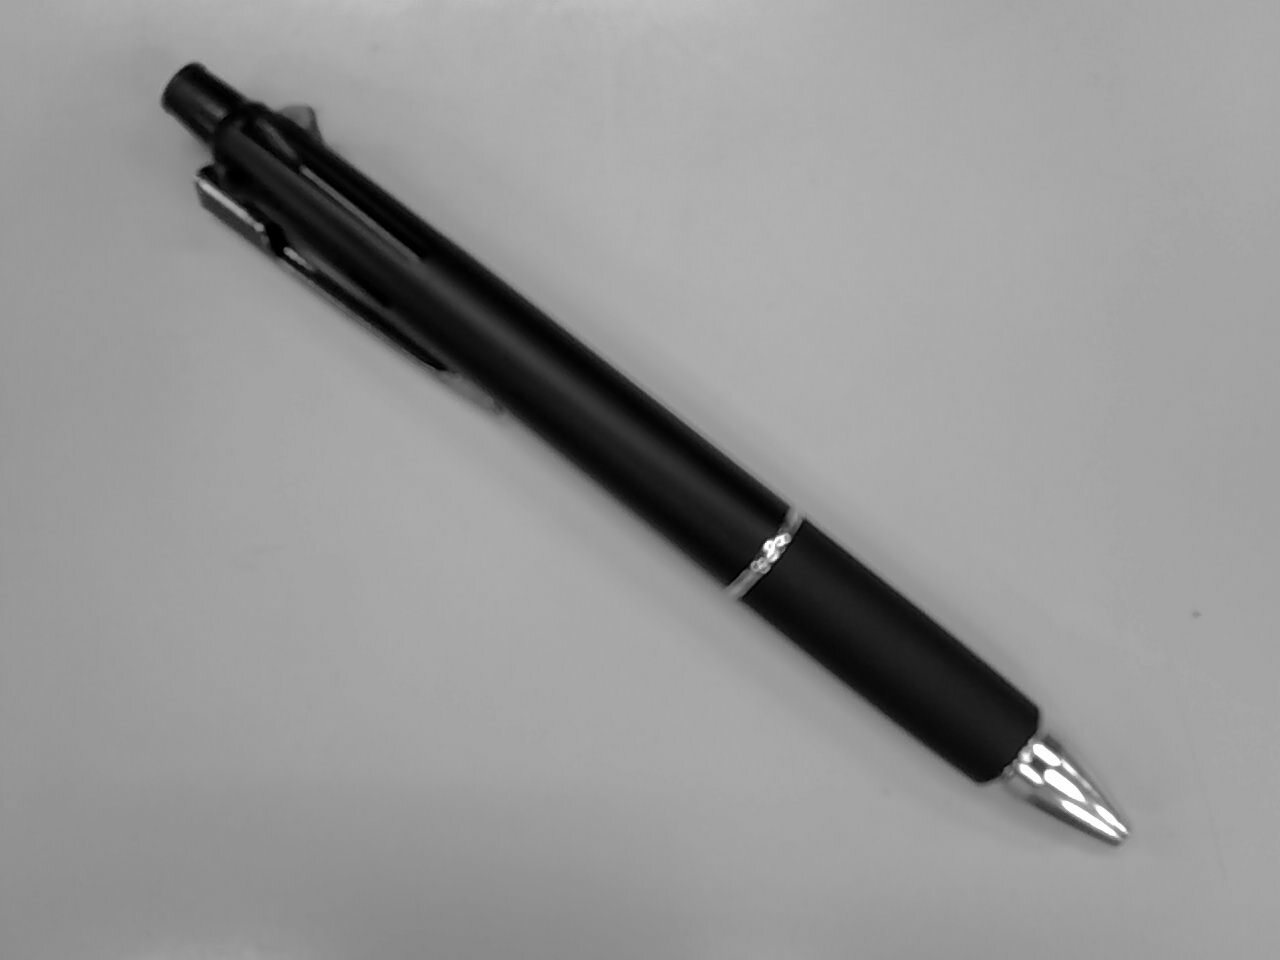
\includegraphics[width=\linewidth]{Image/img_org.png}
		\caption{元画像} \label{fig:img_org}
	\end{minipage}
	\hfill
	\begin{minipage}{0.23\linewidth}
		\centering
		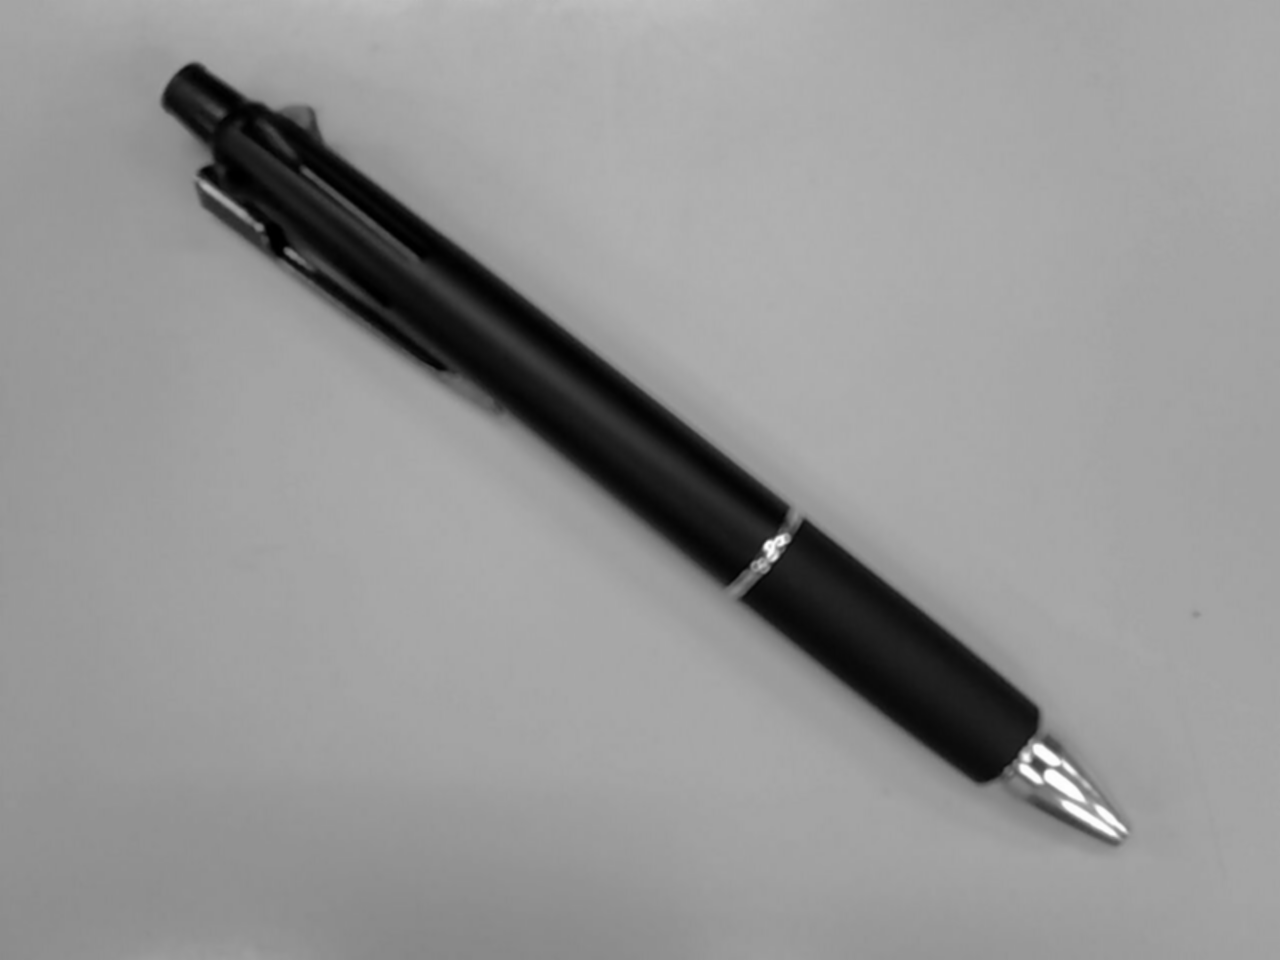
\includegraphics[width=\linewidth]{Image/img_ave.png}
		\caption{平滑化フィルタ後}
	\end{minipage}
	\hfill
	\begin{minipage}{0.23\linewidth}
		\centering
		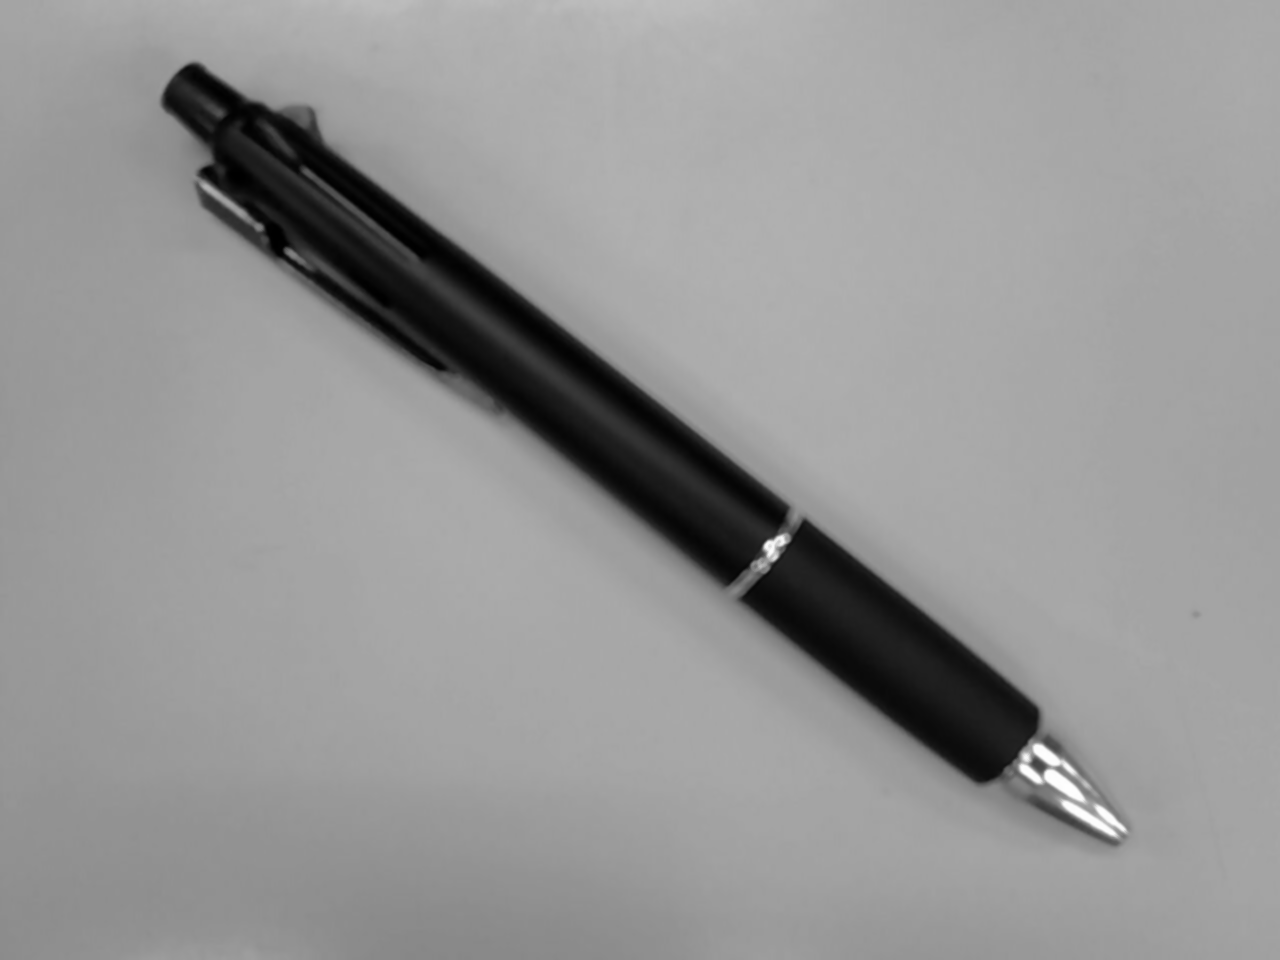
\includegraphics[width=\linewidth]{Image/img_med.png}
		\caption{中央値フィルタ後}
	\end{minipage}
	\hfill
	\begin{minipage}{0.23\linewidth}
		\centering
		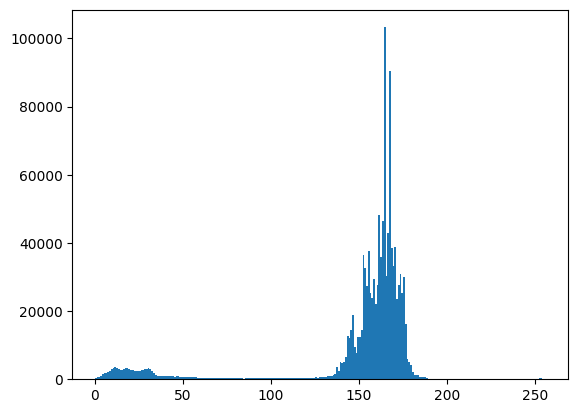
\includegraphics[width=\linewidth]{Image/plt_show.png}
		\caption{ピクセル値のヒストグラム} \label{fig:histgram}
	\end{minipage}
\end{figure}

\begin{figure}[htbp]
	\begin{minipage}{0.23\linewidth}
		\centering
		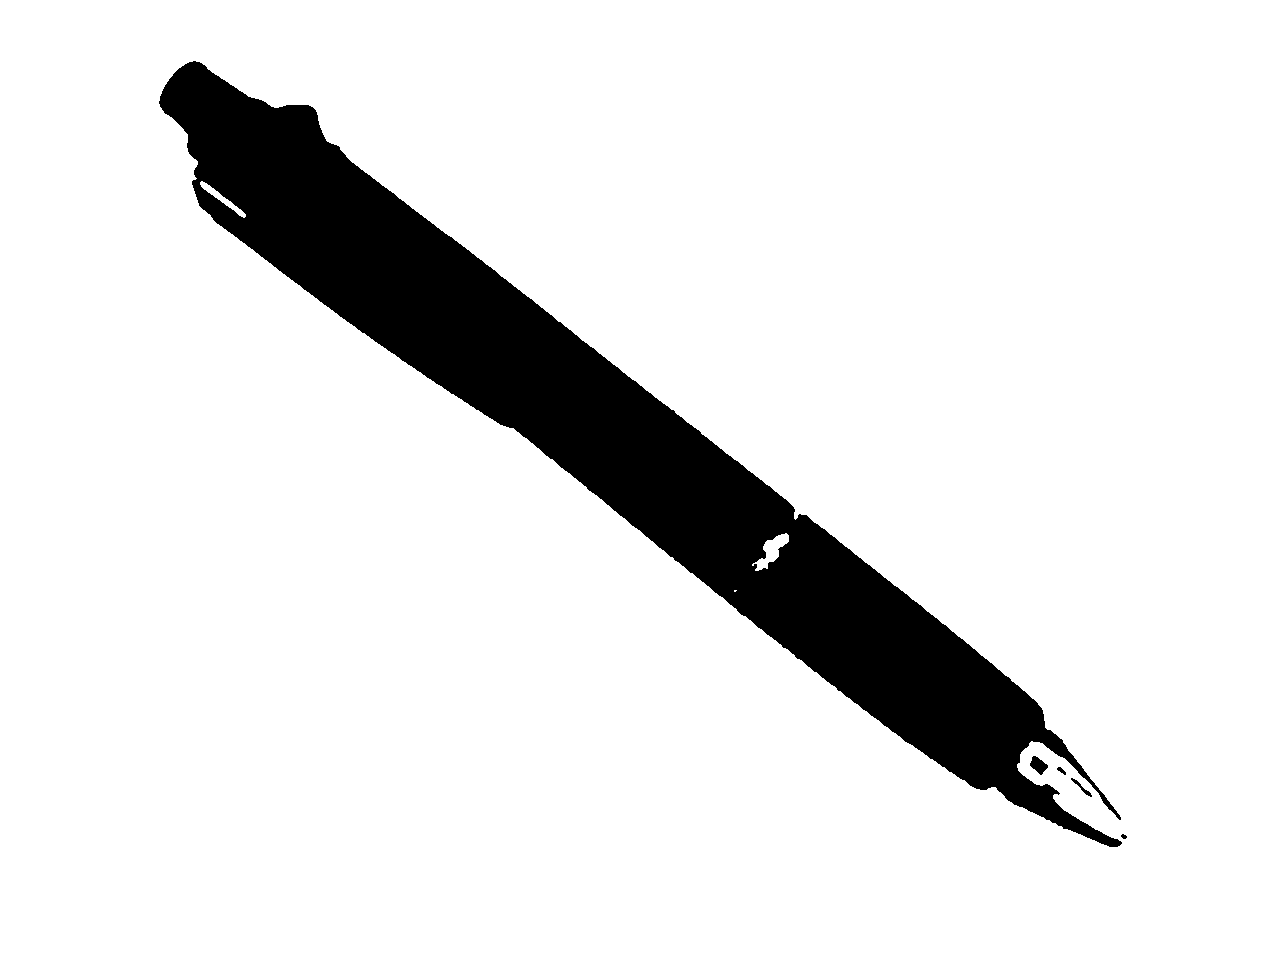
\includegraphics[width=\linewidth]{Image/img_dst.png}
		\caption{二値化後}
	\end{minipage}
	\hfill
	\begin{minipage}{0.23\linewidth}
		\centering
		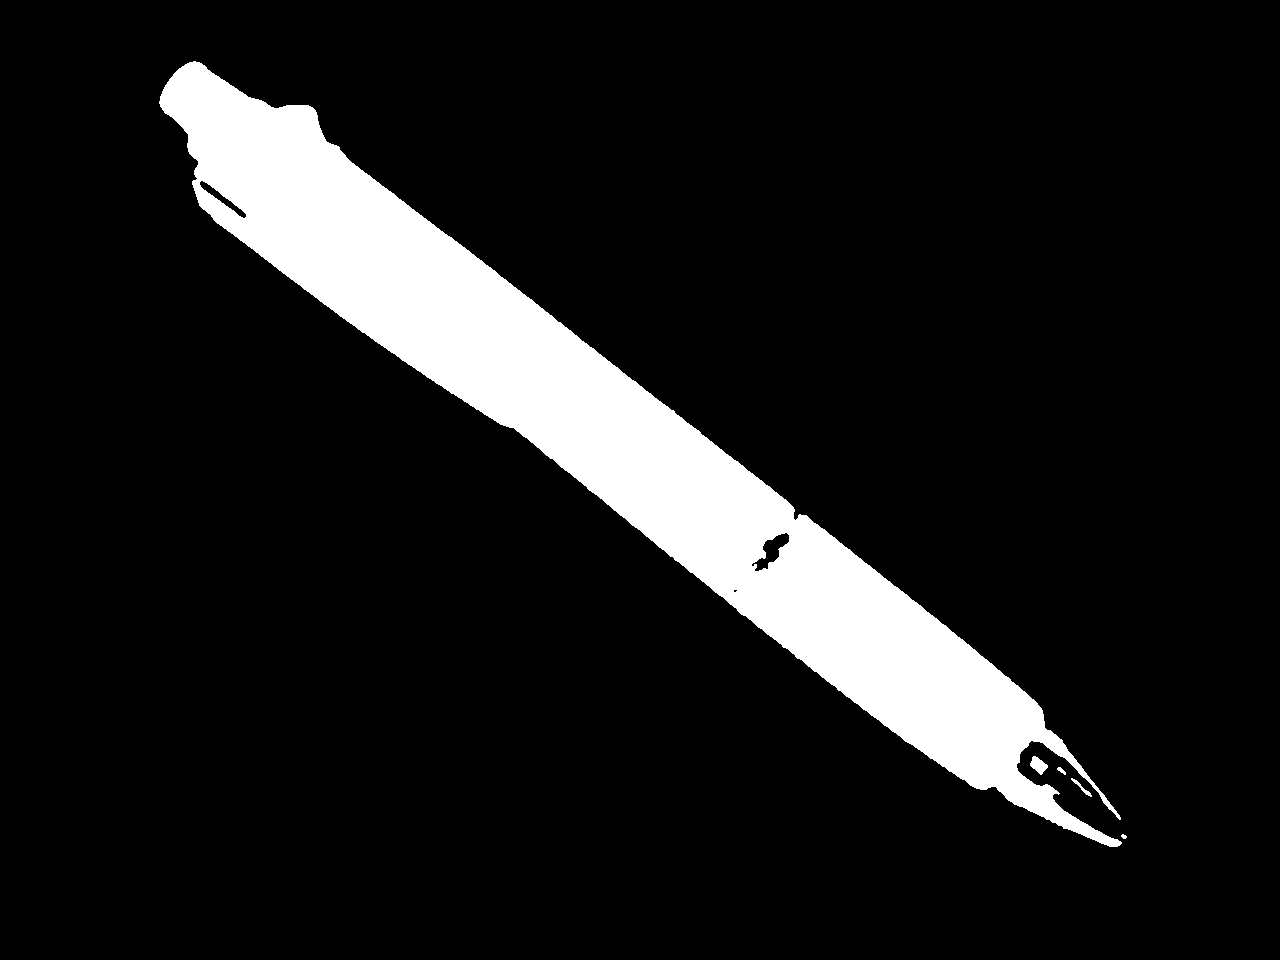
\includegraphics[width=\linewidth]{Image/img_dst2.png}
		\caption{ネガポジ反転後}
	\end{minipage}
	\hfill
	\begin{minipage}{0.23\linewidth}
		\centering
		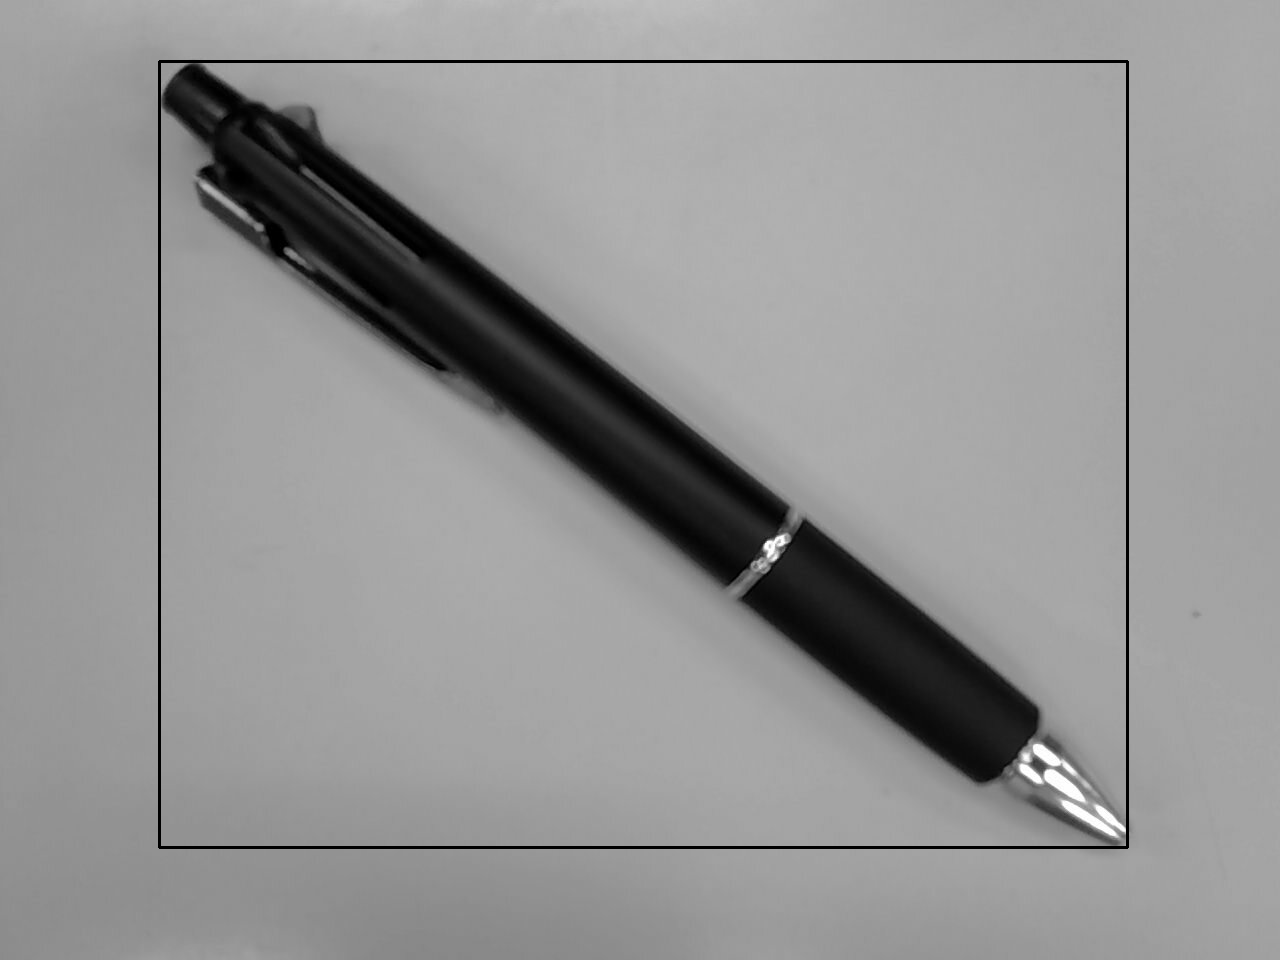
\includegraphics[width=\linewidth]{Image/img_res.png}
		\caption{結果画像} \label{fig:img_res}
	\end{minipage}
\end{figure}

\begin{lstlisting}[caption={物体検出のソースコード},language=Python,label=src:SquareCode]
	import cv2
	import numpy as np 
	from matplotlib import pyplot as plt
	img_org = cv2.imread('Square_org.png',cv2.IMREAD_GRAYSCALE)
	#画像をグレースケール化して読み込み
	img_ave = cv2.blur(img_org,(3,3)) #平滑化フィルタ処理
	img_med = cv2.medianBlur(img_ave,3) #中央値フィルタ処理
	plt.hist(img_med.ravel(),256,[0,256]) #ヒストグラムにプロット
	plt.show() #プロットを表示
	th = 130 #しきい値設定
	ret,img_dst = cv2.threshold(img_med,th,255,cv2.THRESH_BINARY) #二値化処理
	img_dst2 = 255 - img_dst #ネガポジ反転
	x,y,w,h = cv2.boundingRect(img_dst2) #特徴検出
	img = cv2.rectangle(img_org,(x,y),(x+w,y+h),(0,0,0),2) #長方形を描画
	cv2_imshow(img) #結果画像を表示
\end{lstlisting}

\subsection{円検出}

結果は図\ref{fig:img2_org}~\ref{fig:img2_res}のようになった。ソースコードはコード\ref{src:CircleCode}

\begin{figure}
	\begin{minipage}{0.24\linewidth}
		\centering
		\includegraphics[width=\linewidth]{Image/img2_org.png}
		\caption{元画像} \label{fig:img2_org}
	\end{minipage}
	\hfill
	\begin{minipage}{0.24\linewidth}
		\centering
		\includegraphics[width=\linewidth]{Image/img2_gray.png}
		\caption{グレースケール化後} \label{fig:img2_gray}
	\end{minipage}
	\hfill
	\begin{minipage}{0.24\linewidth}
		\centering
		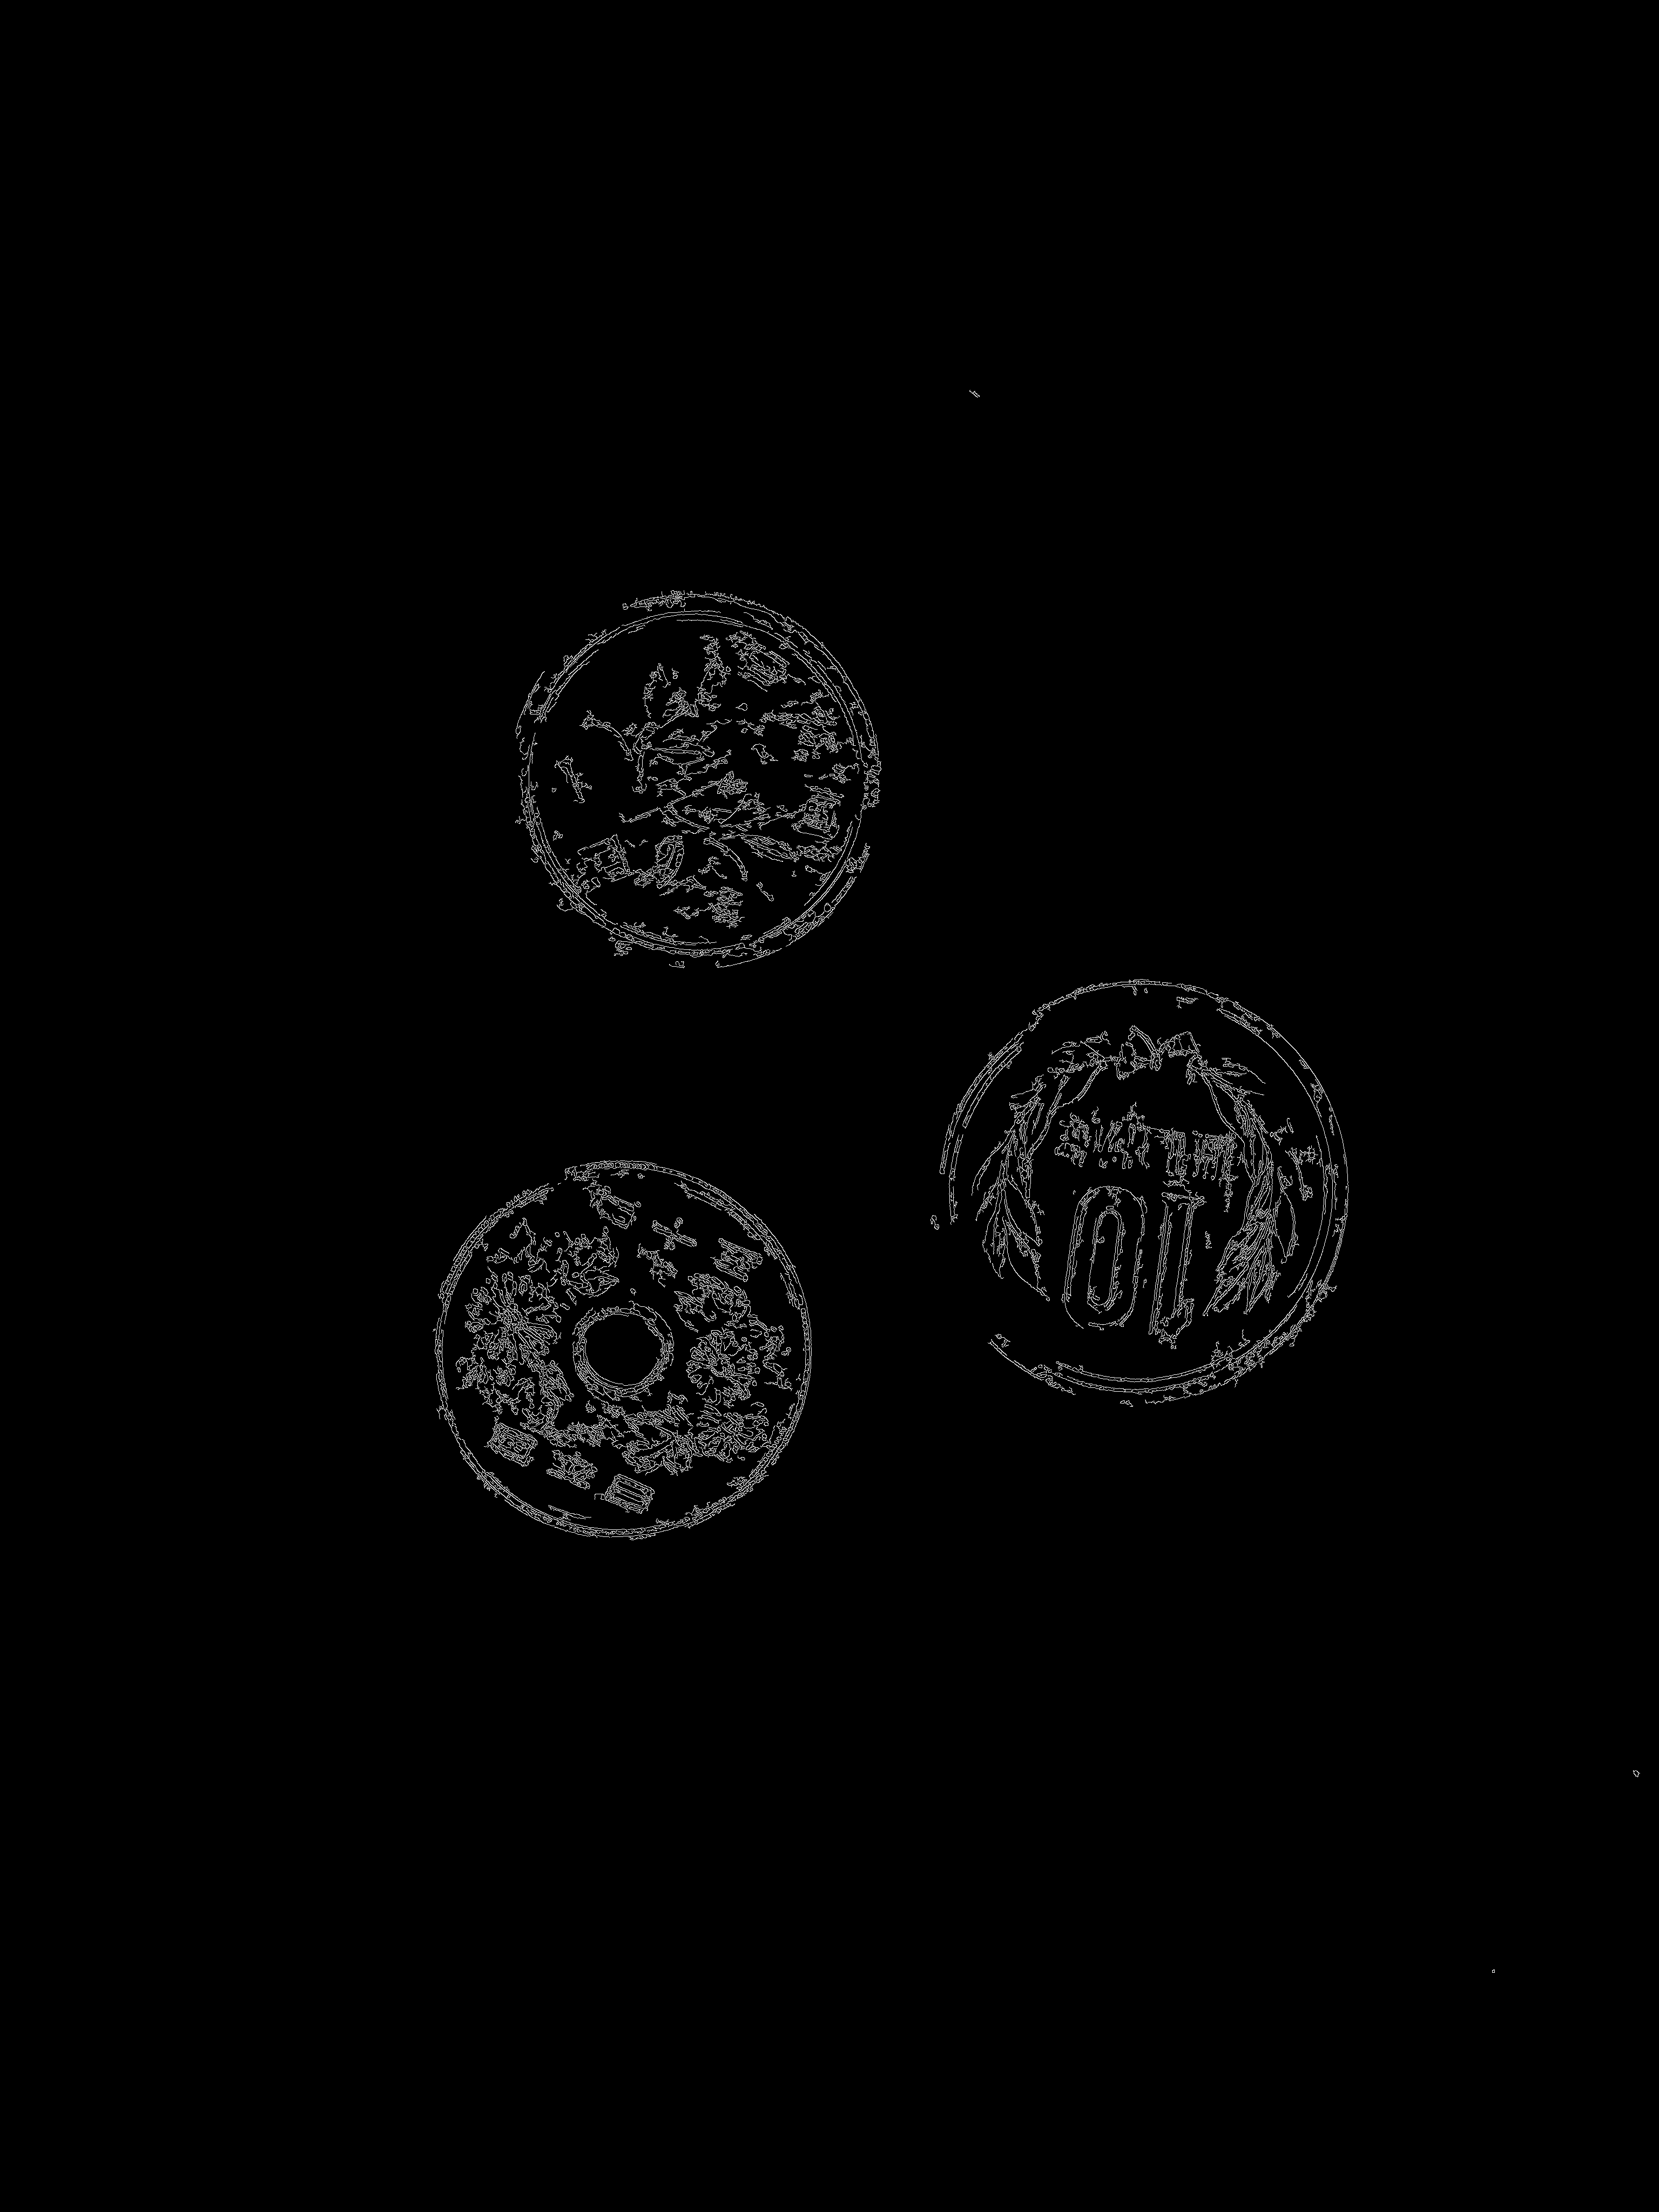
\includegraphics[width=\linewidth]{Image/img2_edge.png}
		\caption{エッジ検出の可視化} \label{fig:img2_edge}
	\end{minipage}
	\hfill
	\begin{minipage}{0.24\linewidth}
		\centering
		\includegraphics[width=\linewidth]{Image/img2_res.png}
		\caption{結果画像} \label{fig:img2_res}
	\end{minipage}
\end{figure}

\begin{lstlisting}[caption={円検出},language=Python,label=src:CircleCode]
	import cv2
	import numpy as np

	img_org = cv2.imread('Circle_org',cv2IMREAD_GRAYSCALE)
	img_edge = cv2.Canny(img_org,10,250)
	img_med = cv2.medianBlur(img_org,3)
	circles = cv2.HoughCircles(image=img_med,method=cv2.HOUGH_GRADIENT,
				dp=2,minDist=100,param1=200,param2=400,
				minRadius=70,maxRadius=400)
	circles = circles.astype('int')
	img_out = img_org.copy()
	for p,q,r in circles[0]:
		cv2.circle(img_out,(p,q),r,(0,255,0),2)
		cv2.circle(img_out,(p,q),5,(255,0,0),5)
	cv2.imshow(img_out)
\end{lstlisting}

\section{考察}

\subsection{物体検出}
\subsubsection{実験1}
\(3\times3\)から\(7\times7\)にしたらよりピクセル値が均一になった。
ピクセル値がすべて3桁の数字になった。

\subsubsection{実験2}
しきい値が150だとノイズが入った。

図\ref{fig:histgram}より130くらいから増えていたのでしきい値を130にした。

長方形がしっかりとボールペンの先端とキャップ側を囲えていた。

\subsubsection{実験3}
結果は表\ref{tb:Jikken3}のようになった。
\begin{table}[htbp]
	\centering
	\caption{実験3の結果}
	\scalebox{0.55}{
		\begin{tabular}{|l|l|l|l|l|l|} \hline
			\multicolumn{2}{|c|}{\multirow{2}{*}{}} & \multicolumn{4}{|c|}{(第1引数,第2引数)}                                                                              \\ \cline{3-6}
			\multicolumn{1}{|c}{}                   &                                   & (低,低)         & (低,高)                & (高,高)        & (高,低)                \\ \hline
			\multirow{2}{*}{第1引数と第2引数の差}            & 近い                                & ノイズ多い。変な箇所あり。 & \(\times\)           & ノイズ少ない。輪郭が変。 & \(\times\)           \\ \cline{2-6}
			                                        & 遠い                                & \(\times\)    & ノイズ少ない。輪郭はしっかりとしている。 & \(\times\)   & ノイズ少ない。輪郭はしっかりとしている。 \\ \hline
		\end{tabular} \label{tb:Jikken3}
	}
\end{table}

\subsection{実験4}
最初50円玉の中心だけが複数個検出された。
なのでminDistとminRadius、maxRadiusを上げた。

すると変な検出がいくつか出てきた。
なのでparam1=100、param2=200、maxRadius=400煮上げた。

するとコインの外側だけを検出することができた。

\section{課題}
\subsection{フィルタ処理について、他にどんな物があるか調査せよ\cite{Highpath}}
\subsubsection{ハイパスフィルタ}
高周波数成分は残し、低周波数成分は除去するようなフィルタをハイパスフィルタという。
周波数成分とは画像の急激な変化のことである。
低周波数を除去し高周波数は残すので、画像のエッジや細かい模様を強調することができる。

\subsection{物体や園の特徴の検出以外に、他にどんなものがあるか調査せよ}
\subsubsection{傾き補正}
画像の文字や文字行の傾きを最小外接矩形を使うとOpenCVのみで傾きの補正が行える。

グレースケール、ノイズ処理、二値化処理をする。
そして文字や文字行を構成するすべての輪郭点をfindContours関数で集める。
集めた点に対してminAreaRect関数を適用し、矩形の回転角度を取得する。
取得した角度を補正角としてgetRotationMatrix2D関数とwarpAffine関数により回転し、水平化する。

これを行うことで画像の文字や文字行の傾きを補正できる。

%\bibliographystyle{plainurl}
%\bibliography{Python1}

\printbibliography

\end{document}
